\chapter{Microsoft Azure}
Platforma została oddana do użytku w 2008 roku jako Windows Azure. Usługa ta została zbudowana na modułach Windows NT. Platforma została udostępniona komercyjnie po 2010 roku, kiedy to dodano możliwość korzystania z szerszej ilości usług i języków programowania. Do usług należało między innymi udostępnienie baz danych Microsoft SQL Server opartych o .NET Framework 4; obsługę aplikacji pisanych w języku C\#, Java, PHP; sieć dostarczania zawartości\trans{ang. Content Delivery Network} (\textbf{CDN}).
\\ \\
Następnym krokiem było przemianowanie platformy na Microsoft Azure oraz pójście w kierunku infrastruktury definiowanej jako serwis\trans{ang. Infrastructure-as-a-Service} (\textbf{IaaS}), oraz powolne adoptowanie usług open-source.
\\ \\
W kolejnej generacji Microsoft zaadoptował rozwiązania Big Data do swojej platformy, umożliwiając korzystanie z języka \textbf{R}, połączenie do Power BI, a także umożliwienie połączenia do rozwiązań end-to-end.
\\ \\
W czwartej generacji platformy, Microsoft skupił się na rozwiązaniach uczenia maszynowego oraz integracji z bazami danych, dzięki czemu powstało Azure Machine Learning Studio oraz Azure Machine Learning Operations (MLOps).
\\ \\
Obecnie platforma została wzbogacona o Kubernetesa, dzięki czemu konteneryzacja ułatwiła pracę z klastrami wirtualnymi, dzięki którym można w lepszy sposób zarządzać aplikacjami i usługami. Dodatkowo zostało udostępnione wiele kombinacji usług takich jak: aplikacja jako usługa \trans{ang. Software-as-a-Service} (\textbf{SaaS}), Interfejs jako usługa \trans{ang. Infrastucture-as-a-Service} (\textbf{IaaS}), Platforma jako usługa \trans{ang. Platfrom-as-a-Service} (\textbf{PaaS}), dzięki czemu uzyskano platformę przyjazną użytkownikowi umożliwiając korzystanie z ponad 200 dostępnych usług. Dodatkowo płatność za platformę jest rozliczana tylko za zużytą przestrzeń oraz wykorzystaną moc obliczeniową.\cite{Roosevelt2022, MicrosoftAzurec, Datashift}.

\begin{figure}[H]
    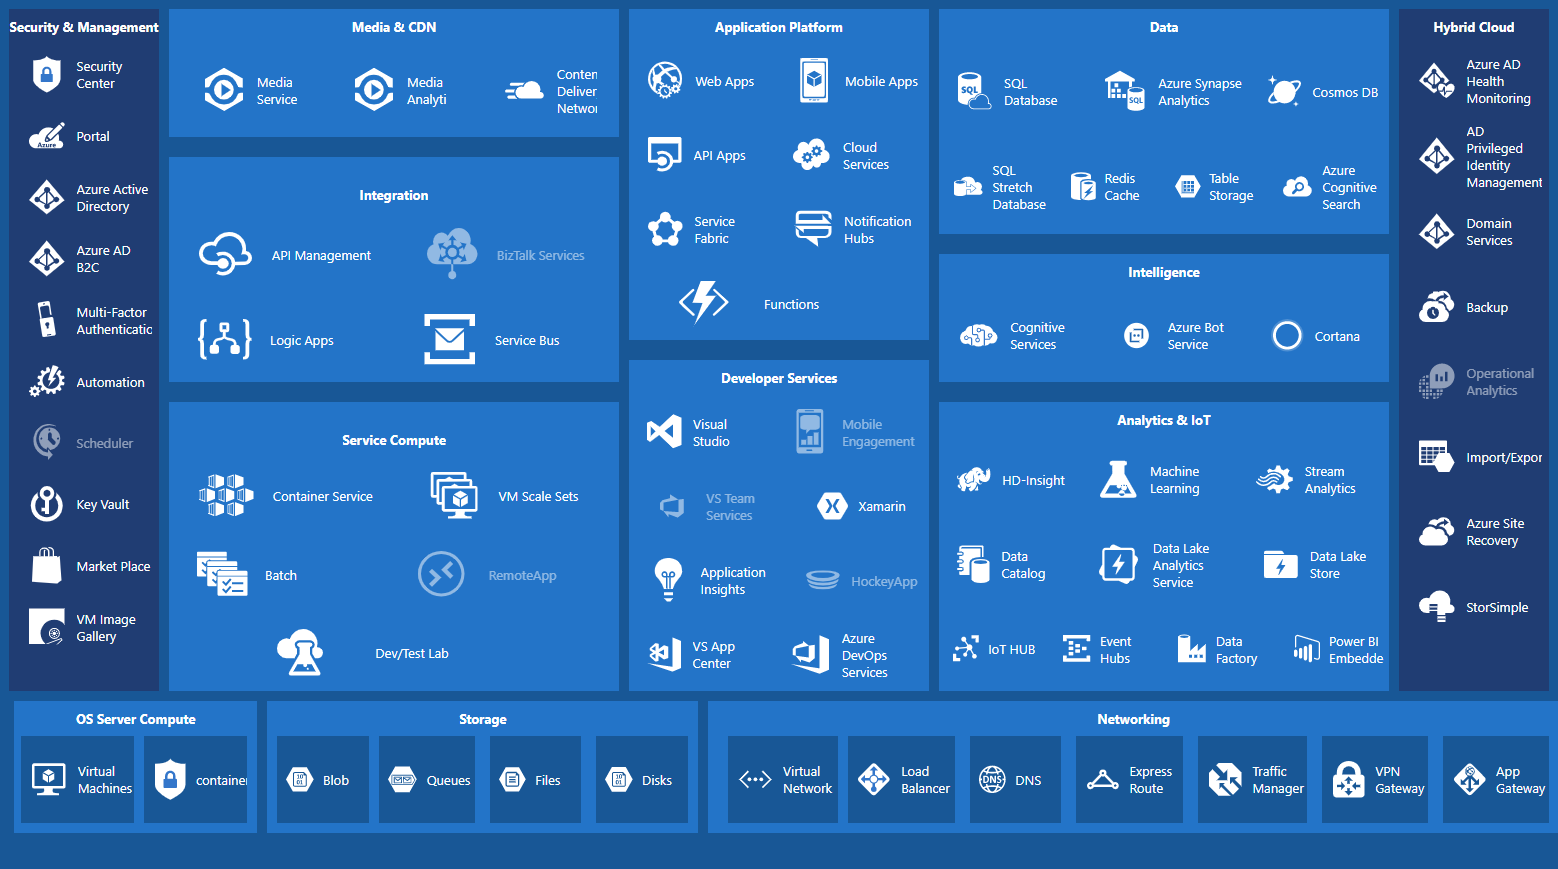
\includegraphics[width=\textwidth]{images/ms_azure}
    \captionsource{Schemat podziału usług MS Azure}{\cite{Datashifta}}
    \label{fig:ms-azure}
\end{figure}

\refsource{Schemat}{fig:ms-azure} pokazuje jak obecnie podzielone są usługi oraz co jest udostępnione komercyjnie w ramach platformy Azure. Według schematu platforma podzielona jest na trzynaście obszarów, do których zaliczono między innymi bezpieczeństwo, zarzazanie danymi, usługi deweloperskie, analiza danych, platformy aplikacji.

\section{Infrastruktura}
Infrastruktura globalna Azure składa się z dwóch części: fizycznej infrastruktury oraz globalnej łączności. Infrastruktura fizyczna składa się z ponad 200 centrów danych na całym świecie, połaczonych w jedną globalną sieć. Dzięki czemu Azure umożliwia wysoką skalowalność i dostępność swoich rozwiązań. Jednakże cały ruch sieciowy jest utrzymywany wewnątrz sieci Microsoft dzięki czemu informacje o adresach IP i ruchu sieciowym nie trafiają do publicznej części internetu\cite{MicrosoftAzureb}.
\\ \\
Na swojej stronie internetowej Microsoft udostępnia wirtualną mapę umożliwiającą zobaczenie na własne oczy jak rozległa jest sieć Microsoftu. Dzięki interaktywności jest możliwość uzyskania informacji o kraju oraz centrum danych, a także komplikacjach jakie wynikają z przepisów wewnętrznych, pokazuje to \refsource{zdjęcie}{fig:azure-ic}.

\begin{figure}[H]
    \begin{subfigure}[m]{0.7\textwidth}
    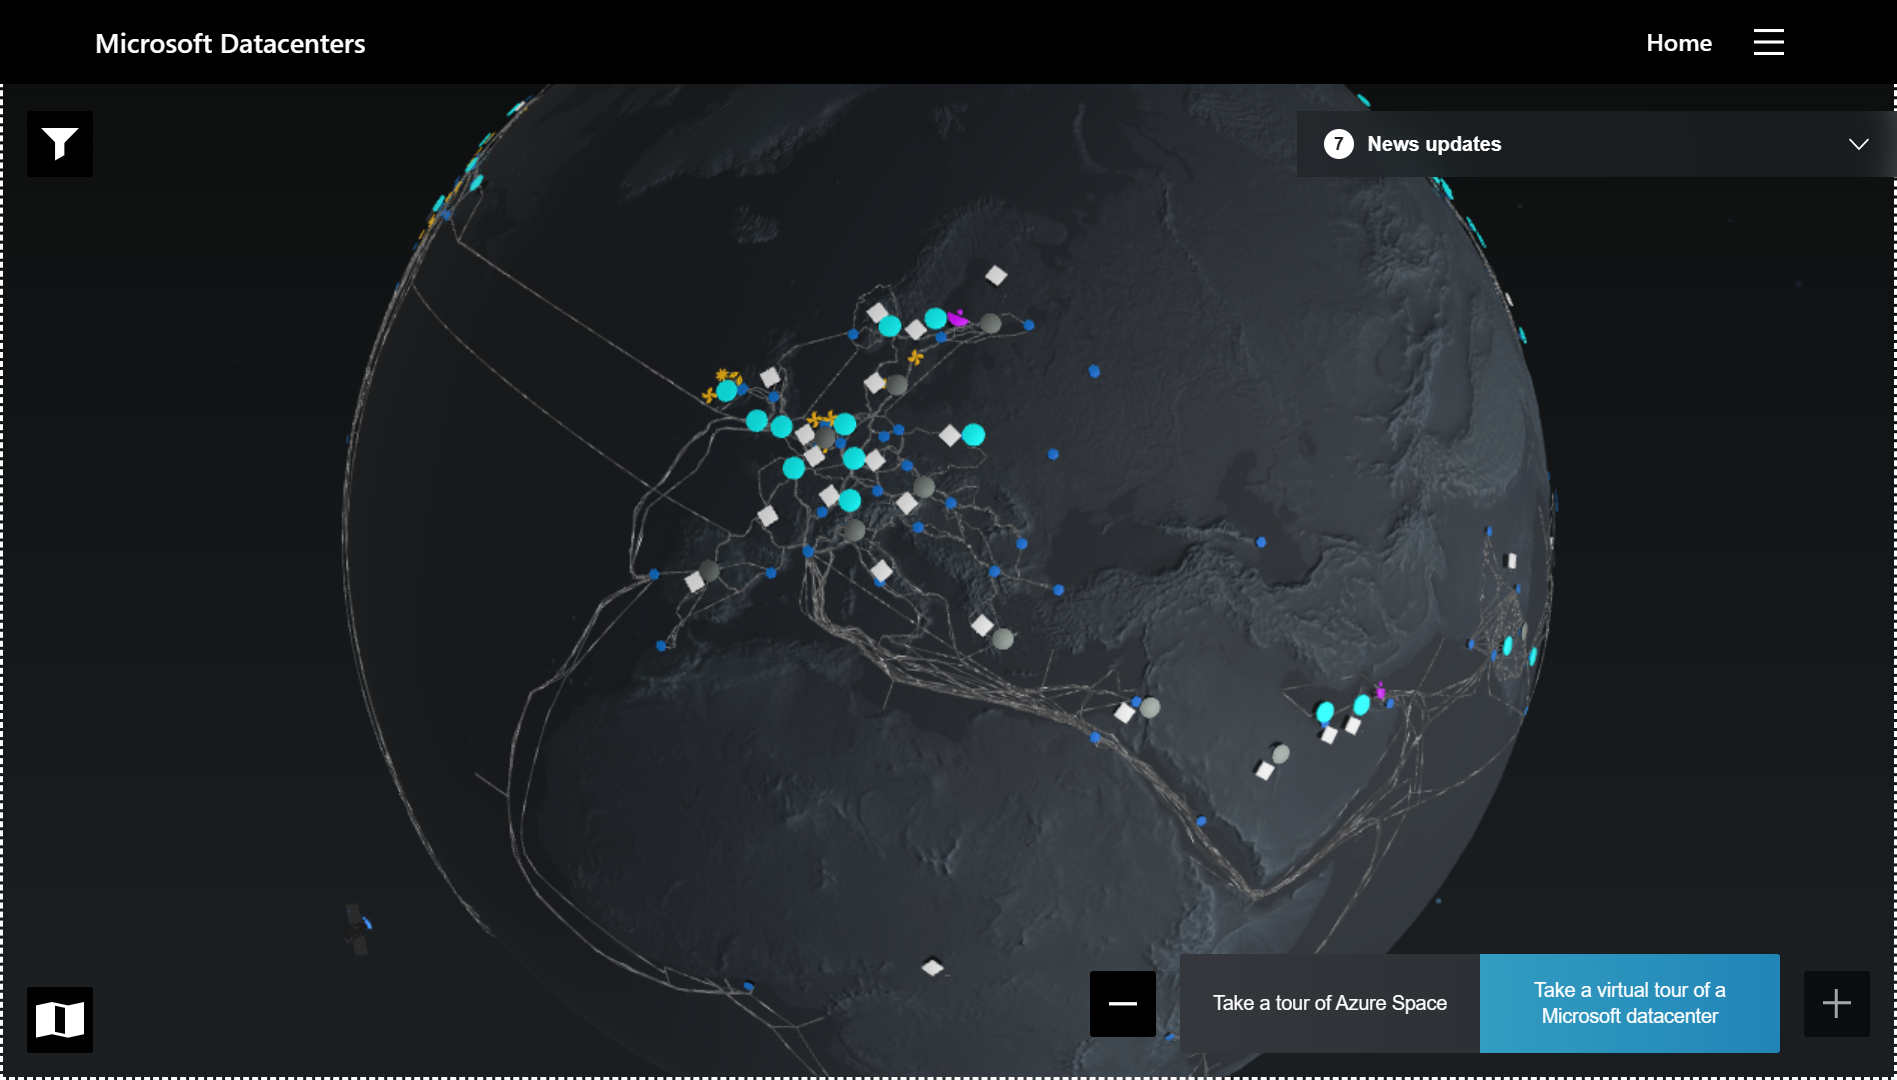
\includegraphics[width=\textwidth]{images/azure-ic}
    \captionsource{Globalna mapa infrastruktury sieciowe}{\cite{MicrosoftAzured}}
    \end{subfigure}
    \hfill
    \begin{subfigure}[m]{0.25\textwidth}
        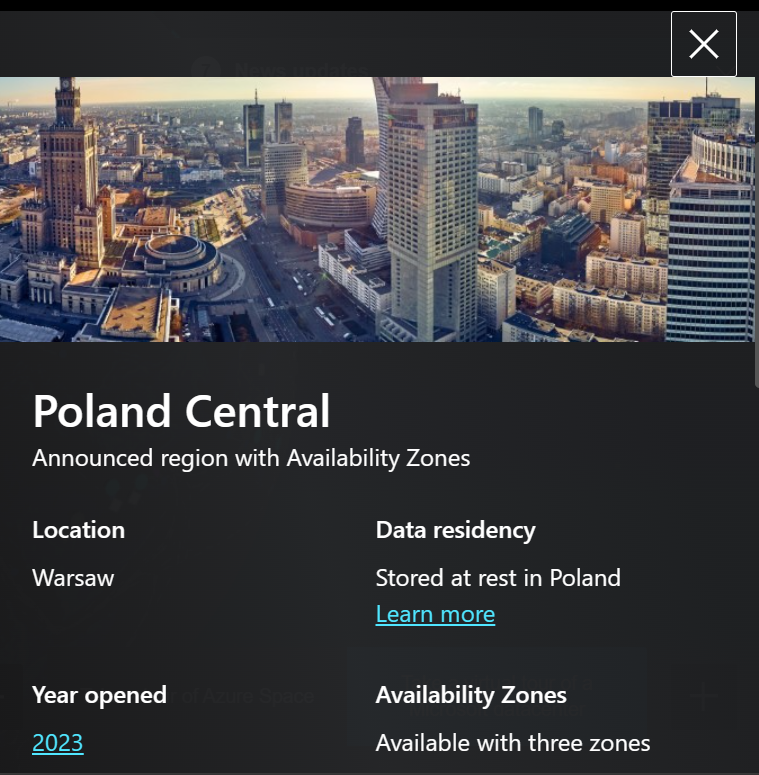
\includegraphics[width=\textwidth]{images/azure-pl}
        \captionsource{Informacje o centrum danych}{\cite{MicrosoftAzuree}}
    \end{subfigure}
    \label{fig:azure-ic}
\end{figure}

\section{Machine Learning Studio}
Azure Machine Learning Studio umożliwia łatwe i szybkie tworzenie wysoce wydajnych modeli uczenia maszynowego, a także zarządzanie nimi. Rozwiązanie wspiera pełen cykl życia kompleksowego uczenia maszynowego. Platforma umożliwia tworzenie potoków zadań, które połączone w jeden potok, wykonują poszczególne zadania w odpowiedniej kolejności. Dzięki modułowości modeli uzyskano rozwiązanie wielokrotnego użytku, a w ramach jednego doświadczenia dany moduł, jeśli nie zostanie zmodyfikowany on, bądź zadania nad nim, zostaje ponownie użyty wynik danego modułu z poprzedniego doświadcenia. Dodatkowo poza predefiniowanymi operacjami można wykorzystać moduły języka Python/R. Dodatkowo można tworzyć rozwiązania w oparciu o ''\textbf{Jupiter Notebook}'', bądź wizualne narzędzie wykorzystujące wizualne układanie ''\textit{kafelek}'' do tworzenia potoków zadań. Dodatkowo każde zadanie wykorzystuje wczesniej przygotowaną jednostkę obliczeniową, dzięki czemu można przewidzieć albo dostosowac koszt korzystania z modelu. Umożliwione zostało również wdrażanie modeli jako punktów końcowych, co umożliwia komunikowanie się z nimi za pomocą REST API.
\\ \\
Microsoft umożliwia płatność jedynie za użytkowanie usług, co oznacza, że jeśli klaster komputerowy był wykorzystywany jedynie przez 1 godzinę, to za tą jedną godzinę zostanie obciążony klient\cite{MicrosoftAzuref}.